\subsection{$K^- d \rightarrow n \pi^+ \pi^- n$ reactions}
\begin{figure}[htbp]
  \centering
  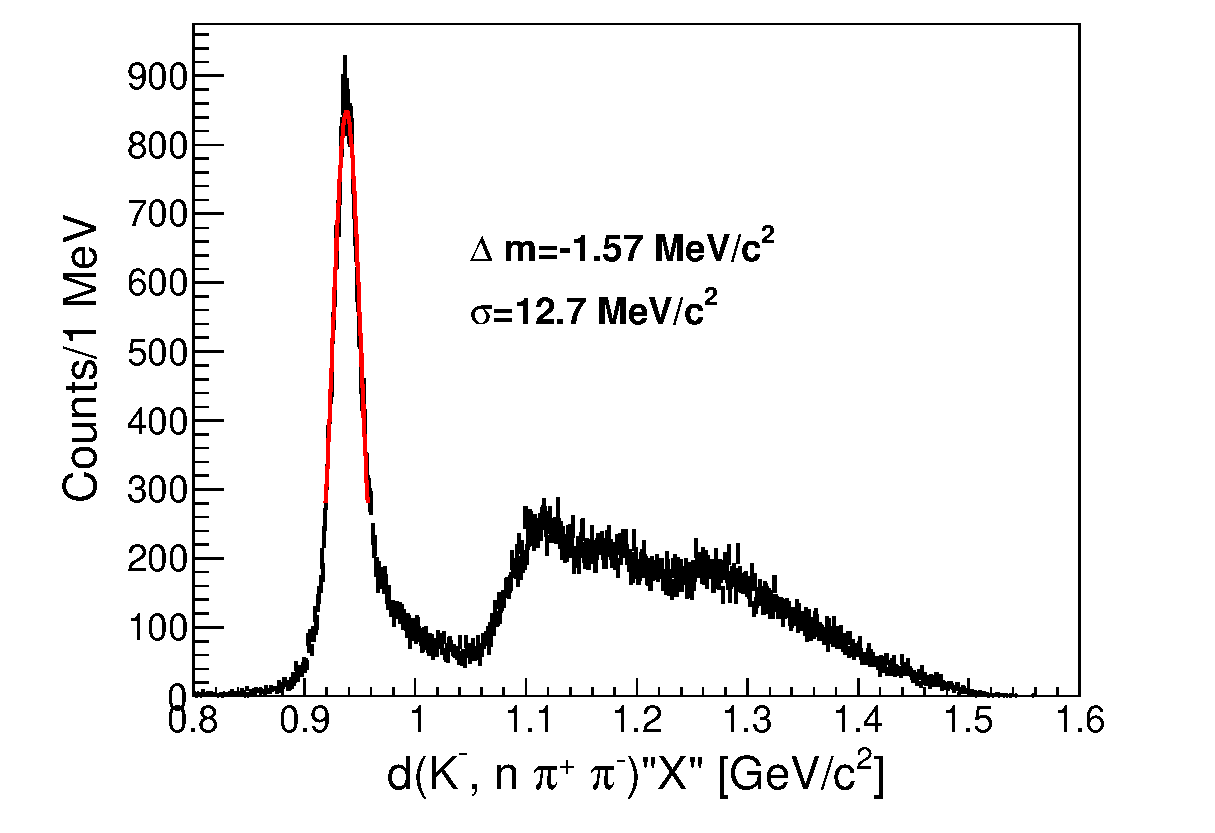
\includegraphics[width=10cm]{../pic/Run78/KN_ana/KNpipi_MM_woFit.eps}
  \caption{
    This figure shows $d(K^-, n \pi^+ \pi^-)"X"$ spectrum.
    Red line indicates fittig gaussian and gray hatched region indicates rejected region for $d(K^-, n \pi^+ \pi^-)"n"$ events.
  }
  \label{fig:KNpipi_MM}
\end{figure}

$K^-d\rightarrow n \pi^+ \pi^- n$ final state was identified in events $n_{forward}$ and $\pi^+ \pi^-$ detected by the NC and the CDS respectively which spectrum was shown in Fig\ref{fig:KNpipi_MM}.
These event selection was adopted offline analysis at seme as $d(K^-, p \pi^- \pi^-)$ analysis which discribed at \ref{sec:software_select_kn}
$d(K^-, n \pi^+ \pi^-)"n"$ events had contamination from materials between rection vertex to the NC.
We adopt 2$\sigma$ selection in $d(K^-, n \pi^+ \pi^-)"n"$ window to avoid the contamination.
The $d(K^-, n \pi^+ \pi^-)"n"$ peak was clearly seen, so we successfully identified $K^- d \rightarrow n \pi^+ \pi^- n$ final state.
The $n$ detected by the NC is called as $n_{detected}$ and the other $n$ is called as $n_{missing}$.\\
In $K^- d \rightarrow n_{detected} \pi^+ \pi^- n_{missing}$ events, three type reactions were expected that shows below.
\begin{enumerate}
\item $K^- d \rightarrow K^0 n n$
\item $K^- d \rightarrow \Sigma^{\pm} \pi^{\mp} n_{missing}$
\item $K^- d \rightarrow \Sigma^{\pm} \pi^{\mp} n_{detected}$
\end{enumerate}
In reaction.1, the $K^0$ can be reconstructed from the $\pi^{\pm}$.
In reaction.2, the neutron decayed from $\Sigma^{\pm}$ is detected.
So, $\Sigma^{\pm}$ can be reconstructed from detected neutron and $\pi^{\pm}$.
These 2 reactions can be identified from detected particles which was indicated in Fig\ref{fig:KNpipi_IM}.
Remained events should be reaction.3.
In this reaction, $K^-$ kicks neutron to forward and strangeness carried to backward and decay to $\pi^{\mp}\Sigma^{\pm}$.
Left figure of Fig.\ref{fig:KN_MM_npipin} shows missing mass of the $d(K^-, n)$ whose final state is identified the $K^- d \rightarrow n \pi^+ \pi^- n$.
$K^0$ and forward-going $\Sigma^{\pm}$ tagged spectra was also shown in same figure.


\begin{figure}[htbp]
  \begin{tabular}{ccc}
    \begin{minipage}{0.33\hsize}
      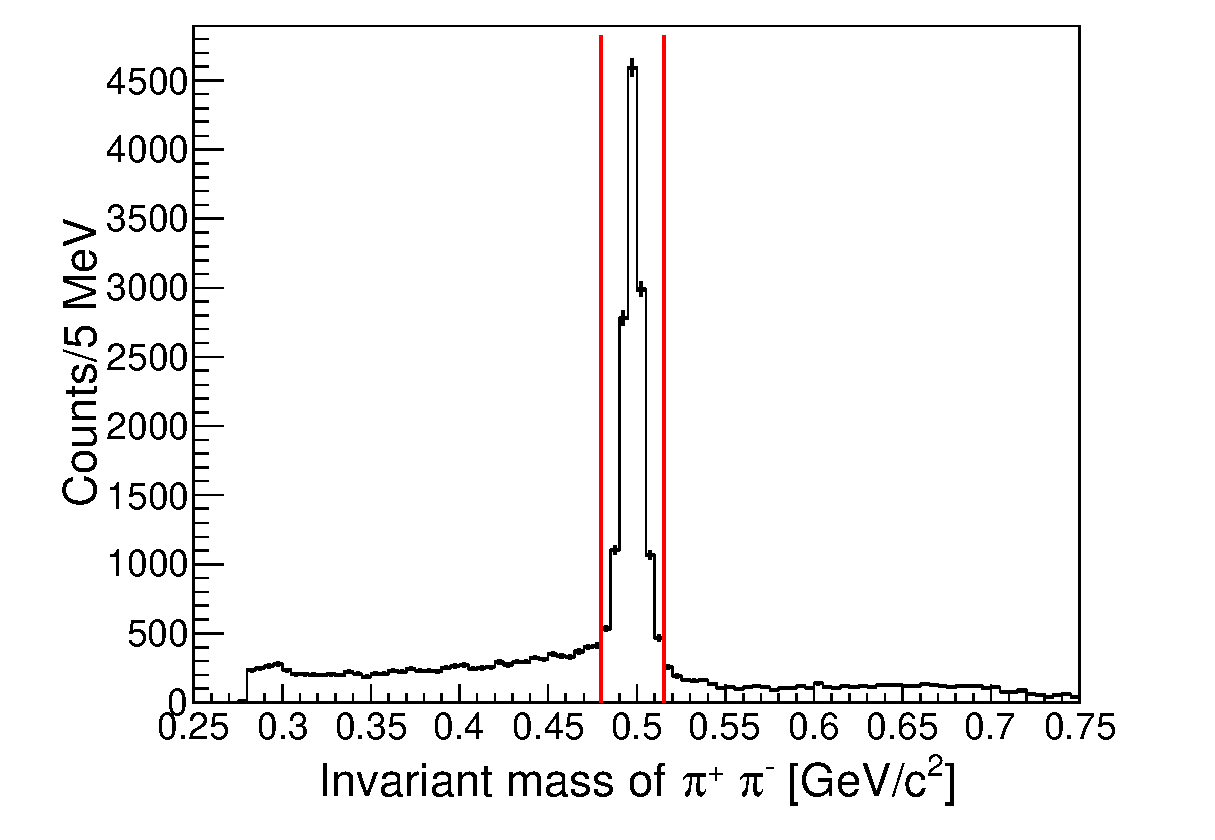
\includegraphics[width=4cm]{../pic/Run78/KN_ana_NC170_2sigma/IM_pipi_woFit.eps}
    \end{minipage}
    \begin{minipage}{0.33\hsize}
      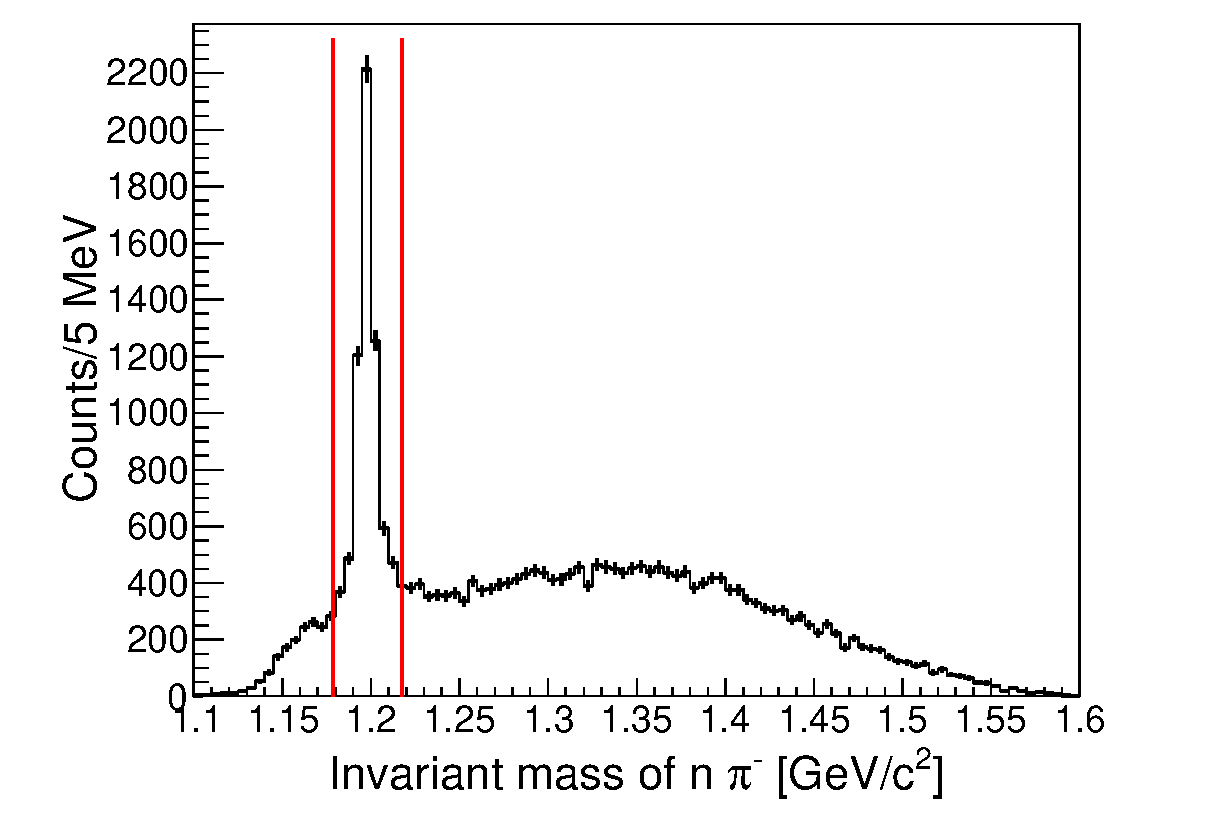
\includegraphics[width=4cm]{../pic/Run78/KN_ana_NC170_2sigma/IM_npim_woFit.eps}
    \end{minipage}
    \begin{minipage}{0.33\hsize}
      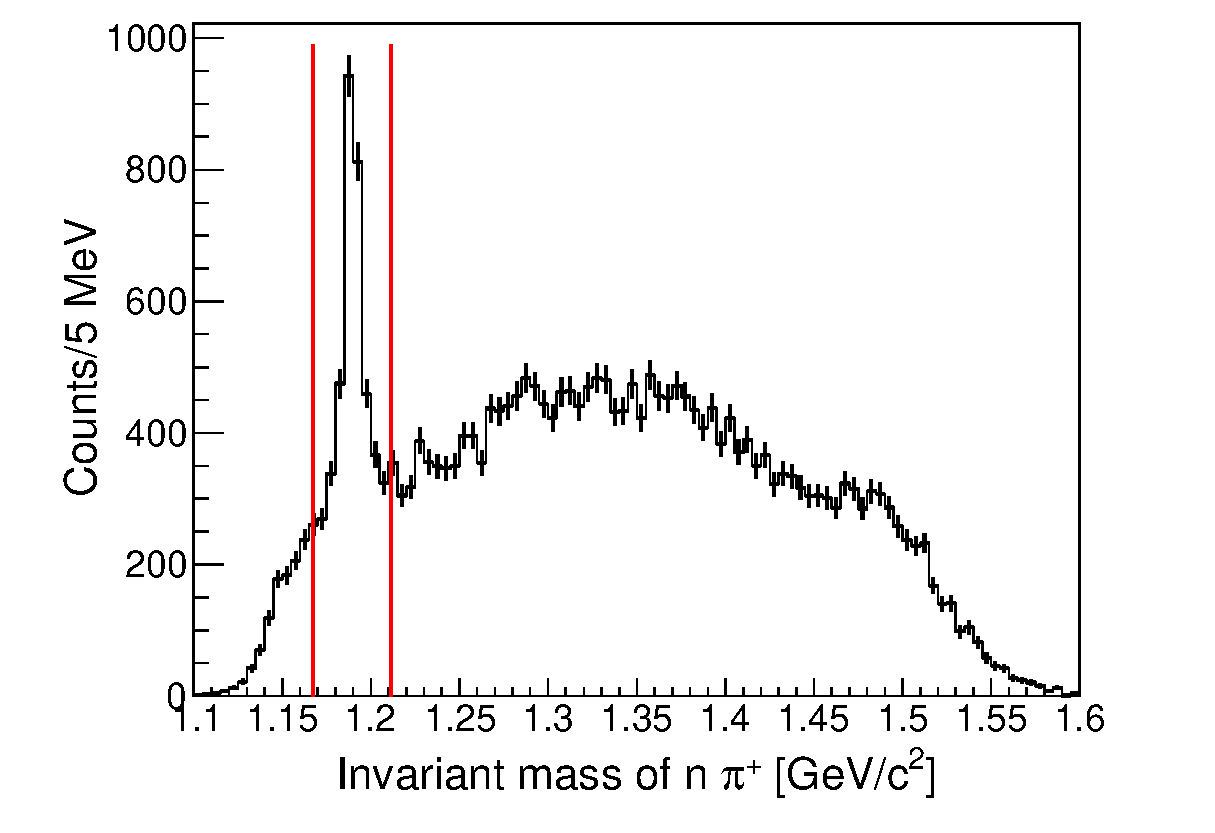
\includegraphics[width=4cm]{../pic/Run78/KN_ana_NC170_2sigma/IM_npip_woFit.eps}
    \end{minipage}
  \end{tabular}

  \caption{
    These figures show invariant masses of $\pi^+ \pi^-$, $n \pi^-$ and $n \pi^+$ in $K^- d \rightarrow n \pi^+ \pi^- n$ final state identified events, respectively.
    Red lines indicate select region for $K^0$, $\Sigma^-_{forward}$ and $\Sigma^+_{backward}$, respectively.
  }
  \label{fig:KNpipi_IM}
\end{figure}

\begin{figure}[htbp]
  \centering  
  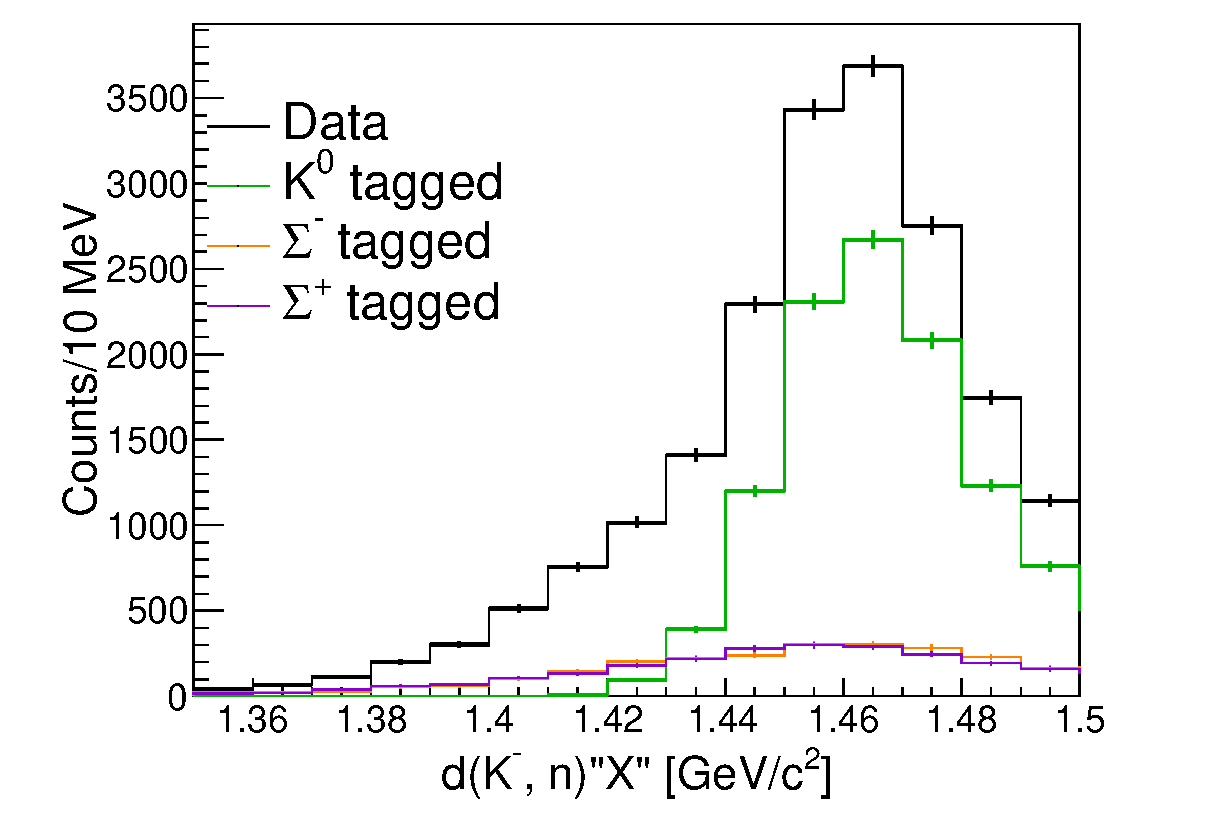
\includegraphics[width=12cm]{../pic/Run78/KN_ana_NC170_2sigma/KN_MM_all.eps}
  \caption{
    This figure shows the missing mass of $d(K^-, n)$ identified $d(K^-, n \pi^+ \pi^-)"n"$ final state.
    Color plots show $K^-$ and $\Sigma_{forward}$ identifed by invariant mass of detected particles.
    $K^0$ contamination is remained in quasi-elastic region.
    $\Sigma_{forward}$ contaminations are negligebly small.
  }
  \label{fig:KN_MM_npipin}
\end{figure}


